%------------------------------------------------------------------------------
\subsection{Installation von Ubuntu}
%------------------------------------------------------------------------------

Nachdem Sie die virtuellen Maschinen gestartet haben, booten diese von dem zuvor angegebenen CD-Abbild. Wählen Sie zunächst die
englische Sprache aus. 
\begin{nofloat}{figure}
\begin{center}
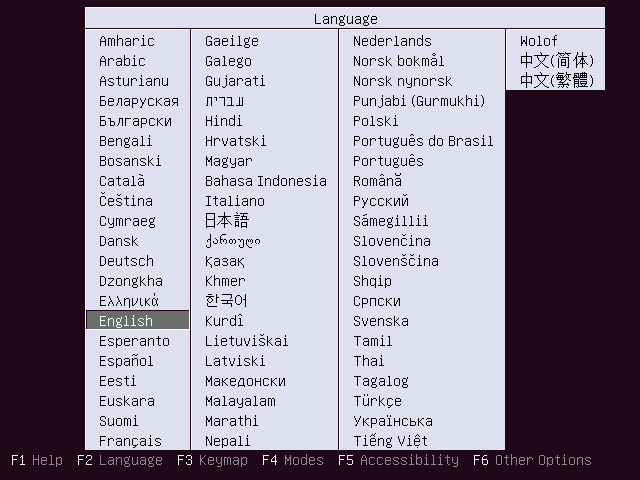
\includegraphics[width=0.70\textwidth]{screenshots/01_ubuntu_install.png}
\end{center}
\end{nofloat}

Danach den Eintrag \textbf{Install Ubuntu Server} wählen und mit der
Eingabe-Taste bestätigen.

\begin{nofloat}{figure}
\begin{center}
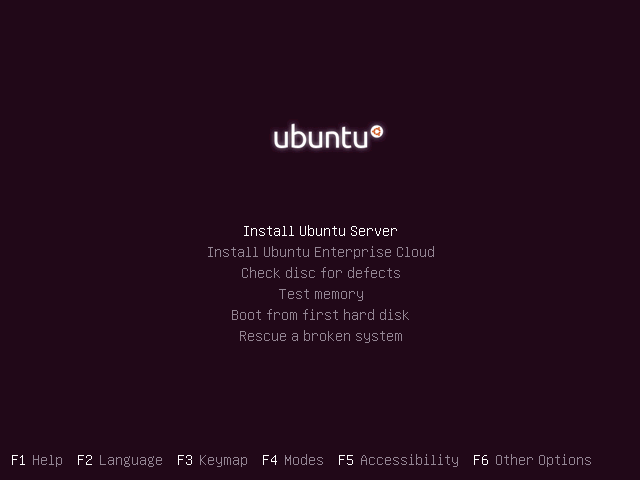
\includegraphics[width=0.85\textwidth]{screenshots/02_ubuntu_install.png}
\end{center}
\end{nofloat}

Um den Installationsprozess in englischer Sprache zu durchlaufen, hier die
Sprache \textbf{English} wählen.

\begin{nofloat}{figure}
\begin{center}
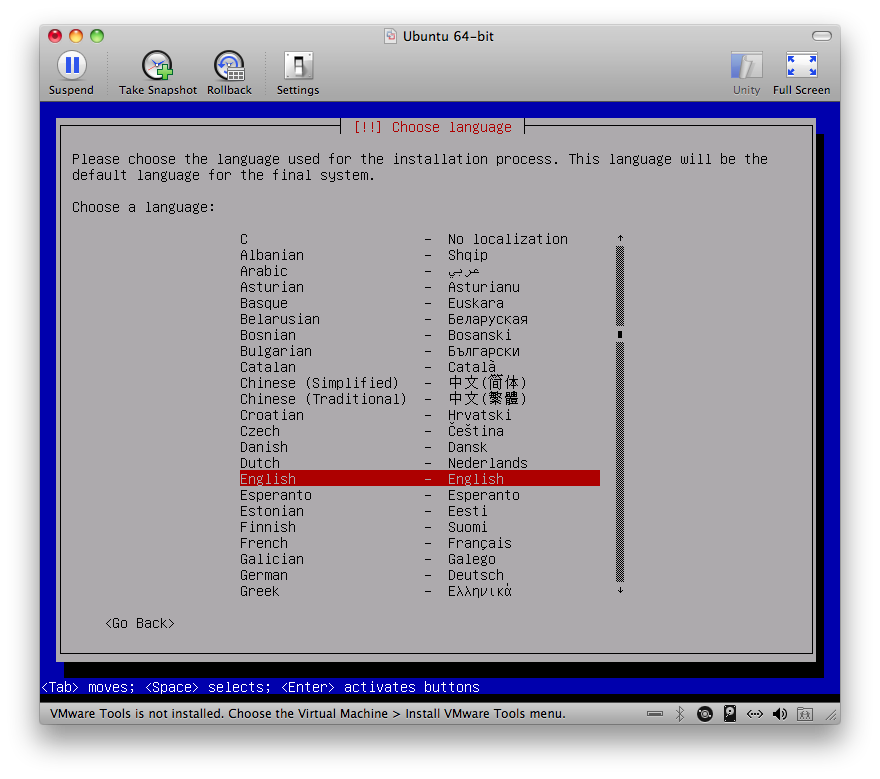
\includegraphics[width=0.85\textwidth]{screenshots/03_ubuntu_install.png}
\end{center}
\end{nofloat}

Die Zeitzone und Region für die Tasturbelegung wird \textbf{Europe} ausgewählt.

\begin{nofloat}{figure}
\begin{center}
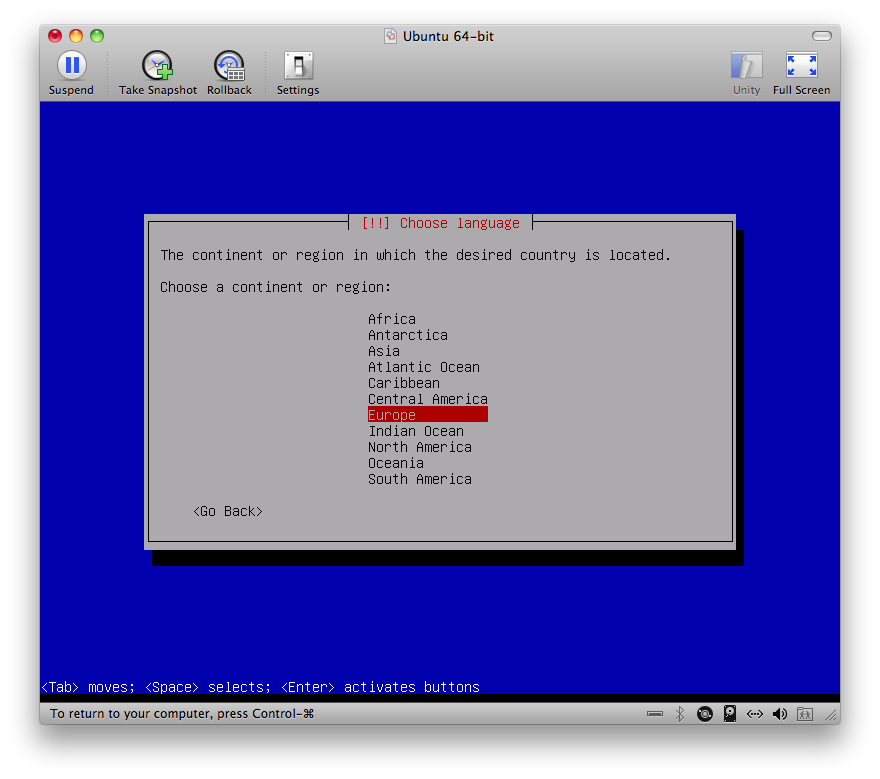
\includegraphics[width=0.85\textwidth]{screenshots/04_ubuntu_install.png}
\end{center}
\end{nofloat}

Im nächsten Dialog als Land \textbf{Germany} auswählen.


BREAK BREAK

Als nächster Schritt wird die Tastatur-Belegung angegeben. Sie können diese automatisch erkennen lassen. Hierzu müssen Sie in
den folgenden Dialogen verschiedene Tasten drücken.

Nach der Hardware- und Netzwerk-Erkennung können Sie nun einen Hostnamen eintragen. Geben Sie hier bitte \textbf{srv1} an.

\begin{nofloat}{figure}
\begin{center}
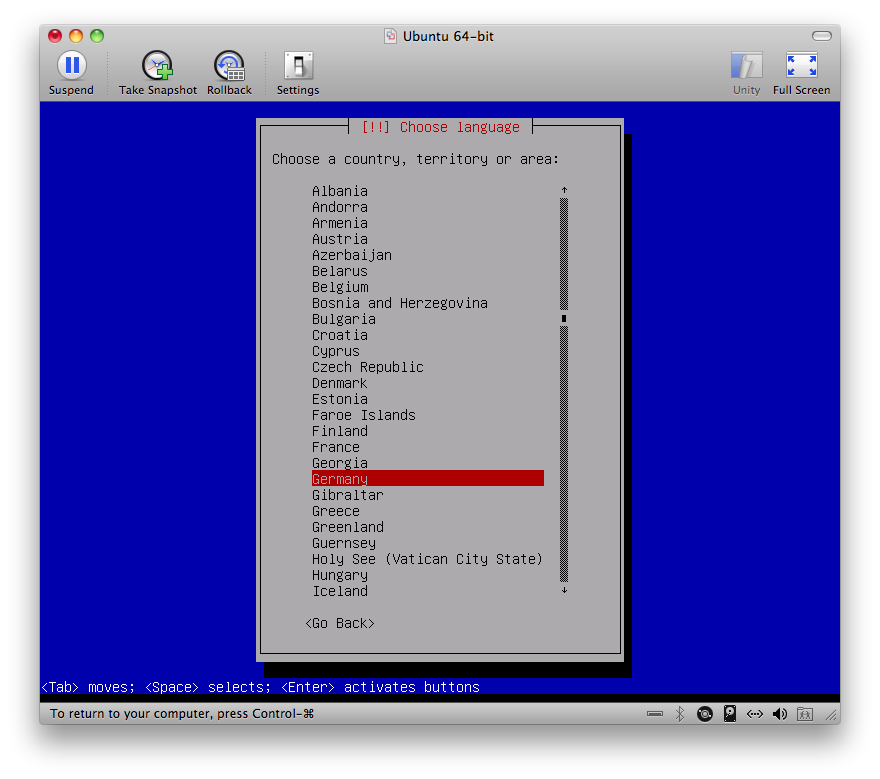
\includegraphics[width=0.85\textwidth]{screenshots/05_ubuntu_install.png}
\end{center}
\end{nofloat}

\pagebreak
Die Zeitzone \textbf{Europe/Berlin} können Sie mit \textbf{Ja} bestätigen.

\begin{nofloat}{figure}
\begin{center}
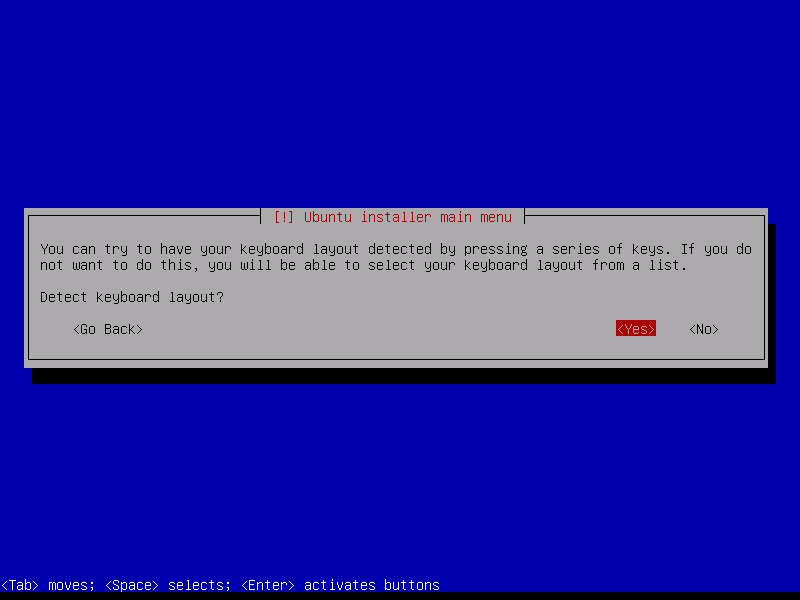
\includegraphics[width=0.85\textwidth]{screenshots/06_ubuntu_install.png}
\end{center}
\end{nofloat}

Nun wird die Festplatte partitioniert. Wählen Sie hier den Eintrag \textbf{Manuell}.

\begin{nofloat}{figure}
\begin{center}
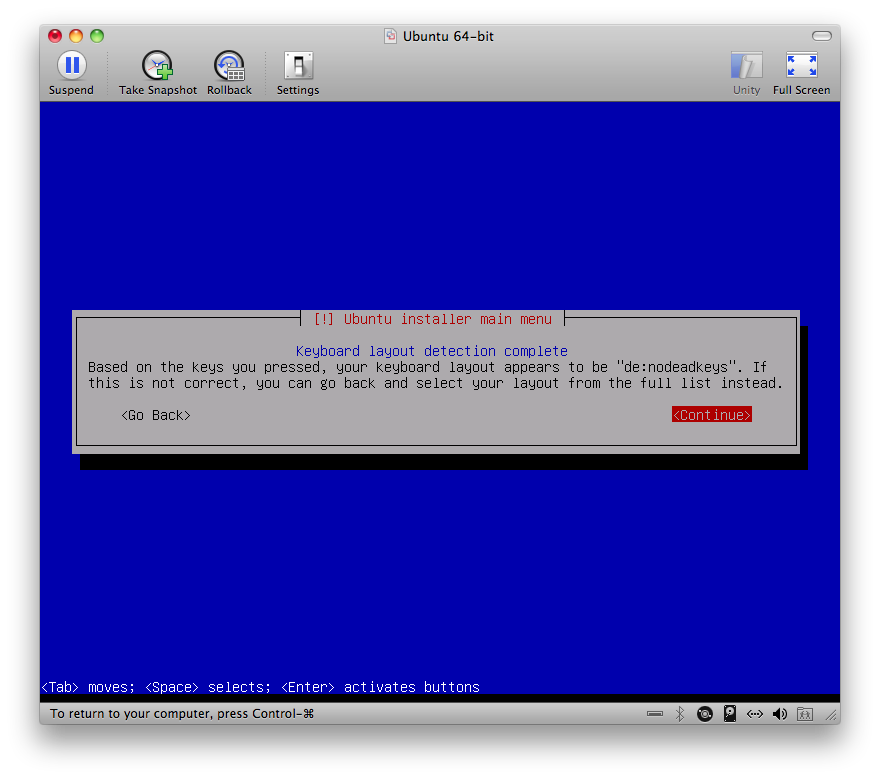
\includegraphics[width=0.85\textwidth]{screenshots/07_ubuntu_install.png}
\end{center}
\end{nofloat}

\pagebreak
Hier nun den Eintrag \textbf{SCSI3} wählen.

\begin{nofloat}{figure}
\begin{center}
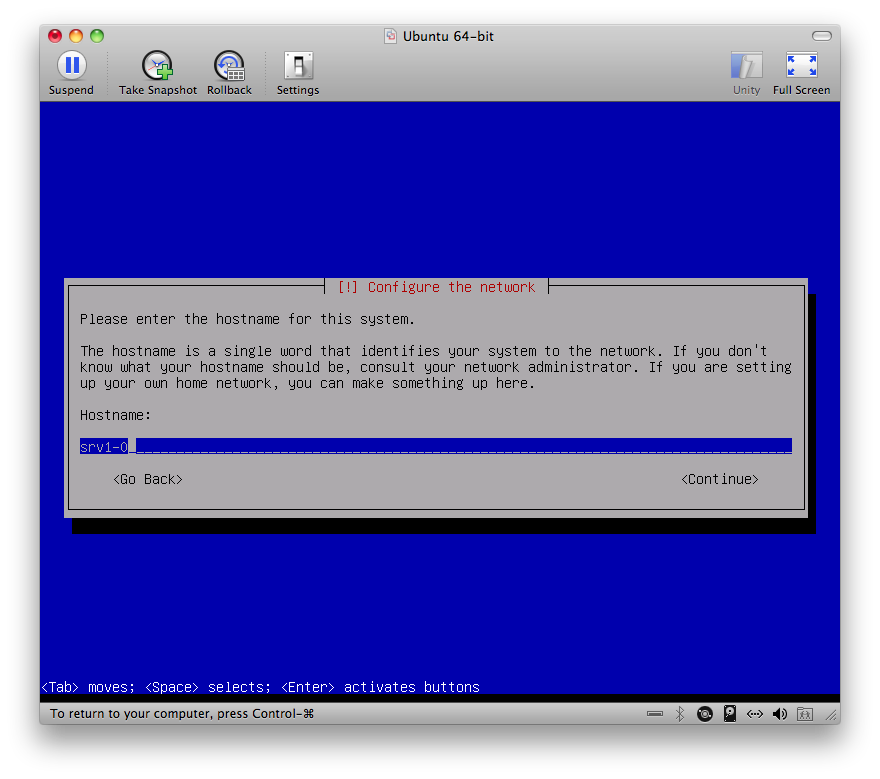
\includegraphics[width=0.85\textwidth]{screenshots/08_ubuntu_install.png}
\end{center}
\end{nofloat}

Erzeugen Sie eine neue leere Partitionstabelle.

\begin{nofloat}{figure}
\begin{center}
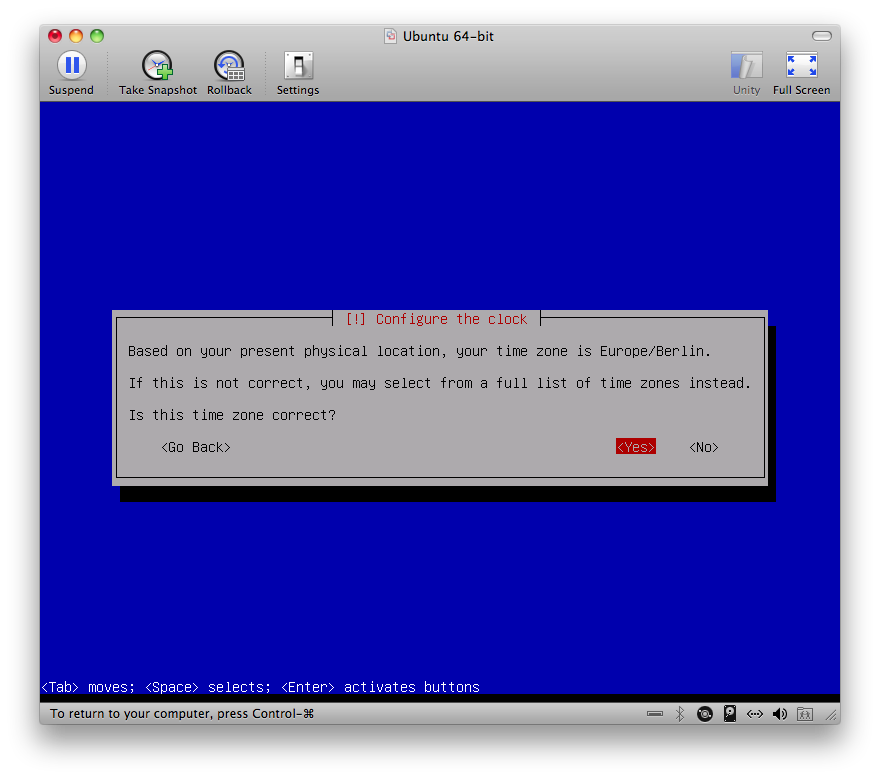
\includegraphics[width=0.85\textwidth]{screenshots/09_ubuntu_install.png}
\end{center}
\end{nofloat}

\pagebreak
Wählen Sie hier nun den \textbf{FREIEN SPEICHER} aus.

\begin{nofloat}{figure}
\begin{center}
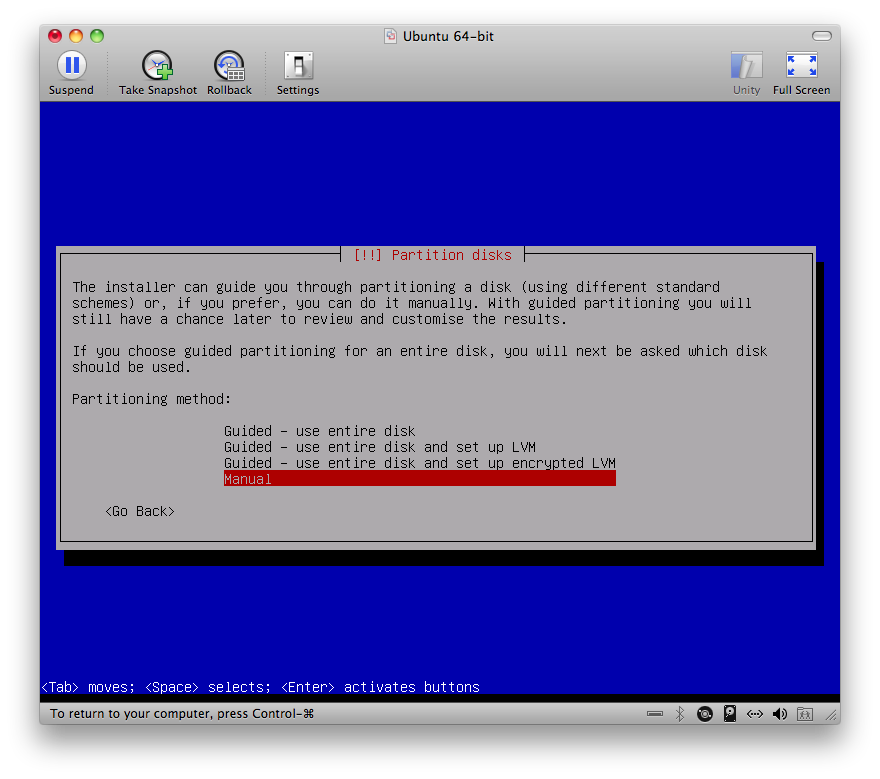
\includegraphics[width=0.85\textwidth]{screenshots/10_ubuntu_install.png}
\end{center}
\end{nofloat}

Hier nun \textbf{Eine neue Partition erstellen} wählen.

\begin{nofloat}{figure}
\begin{center}
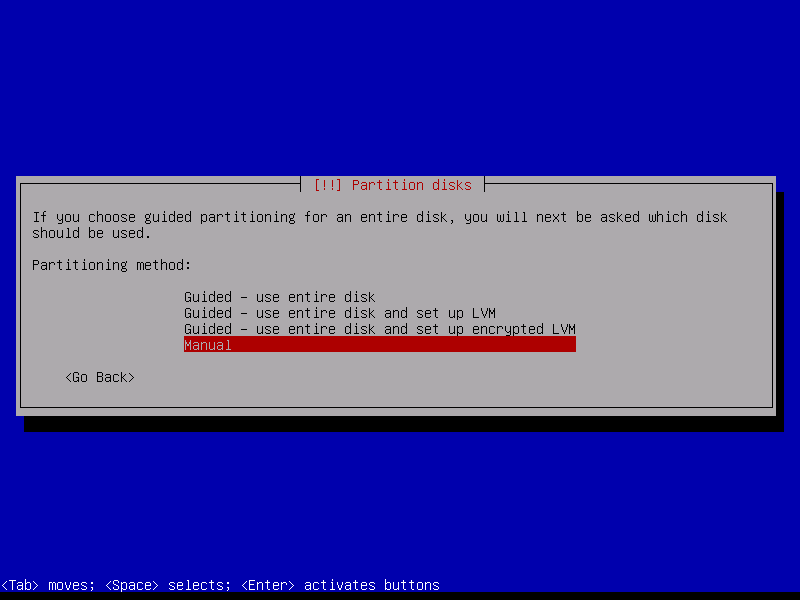
\includegraphics[width=0.85\textwidth]{screenshots/11_ubuntu_install.png}
\end{center}
\end{nofloat}

\pagebreak
Als Größe geben Sie bitte hier \textbf{8.0 GB} an.

\begin{nofloat}{figure}
\begin{center}
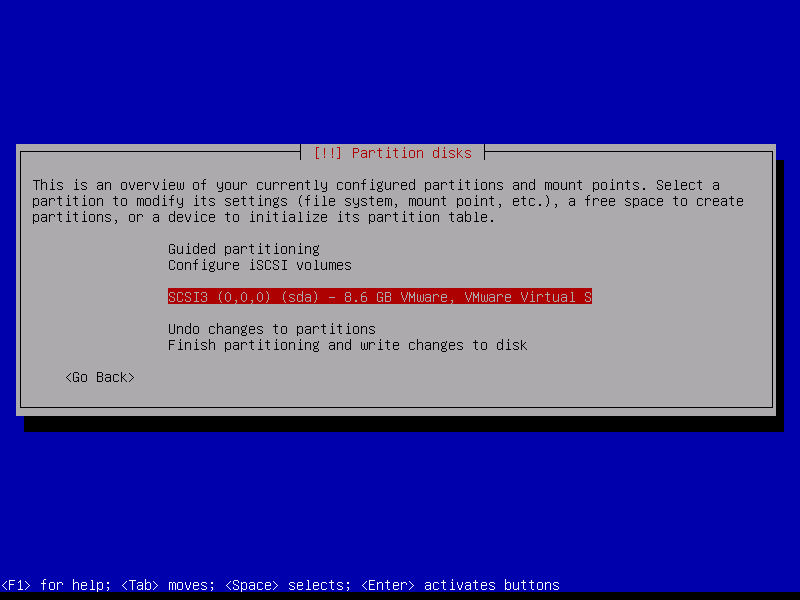
\includegraphics[width=0.85\textwidth]{screenshots/12_ubuntu_install.png}
\end{center}
\end{nofloat}

Hier nun \textbf{Primär} wählen.

\begin{nofloat}{figure}
\begin{center}
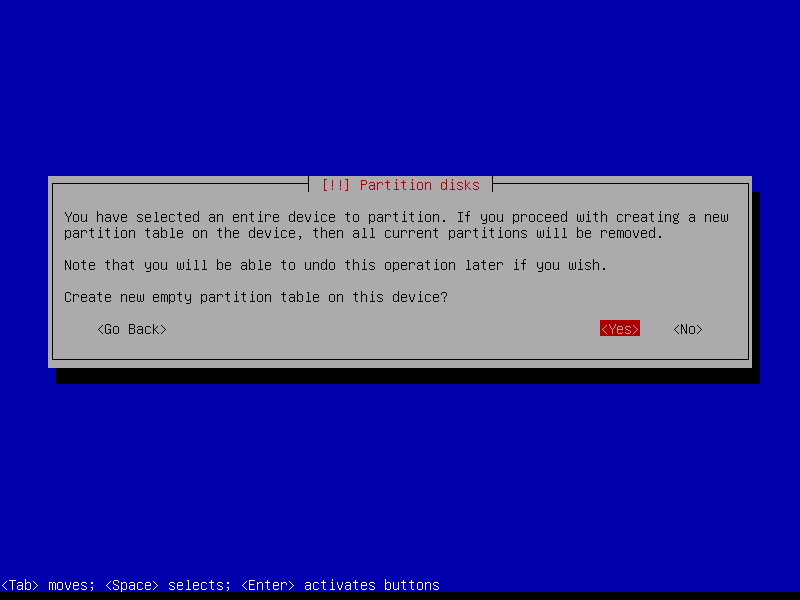
\includegraphics[width=0.85\textwidth]{screenshots/13_ubuntu_install.png}
\end{center}
\end{nofloat}

\pagebreak
Dieser Eintrag ist schon korrekt und kann mit \textbf{Anlegen der Partition beenden} bestätigt werden.

\begin{nofloat}{figure}
\begin{center}
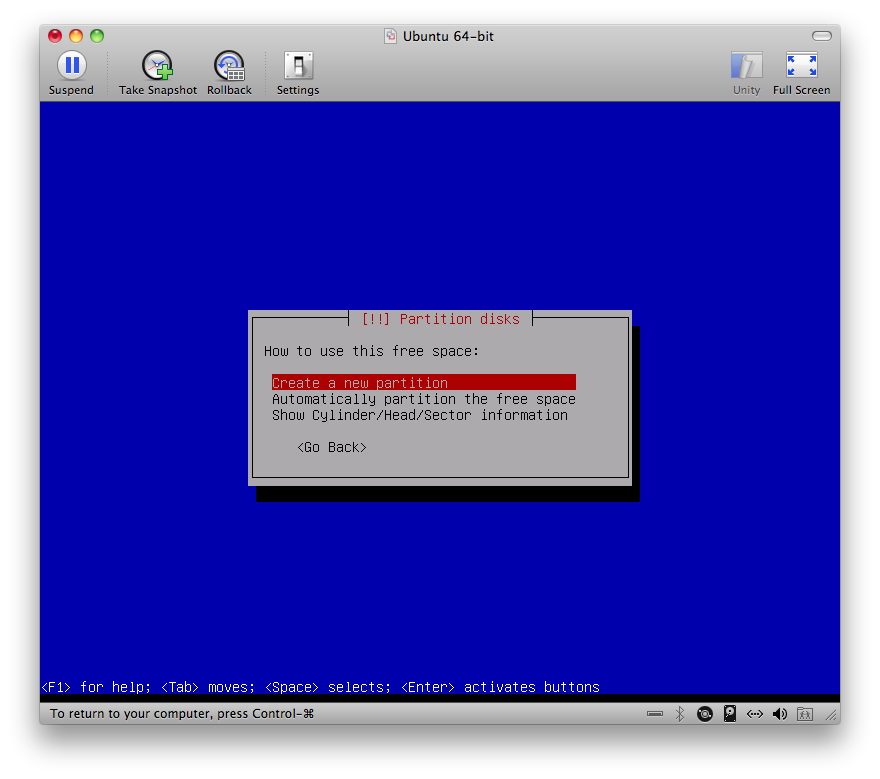
\includegraphics[width=0.85\textwidth]{screenshots/14_ubuntu_install.png}
\end{center}
\end{nofloat}

Wählen Sie hier wiederum \textbf{FREIER SPEICHER}.

\begin{nofloat}{figure}
\begin{center}
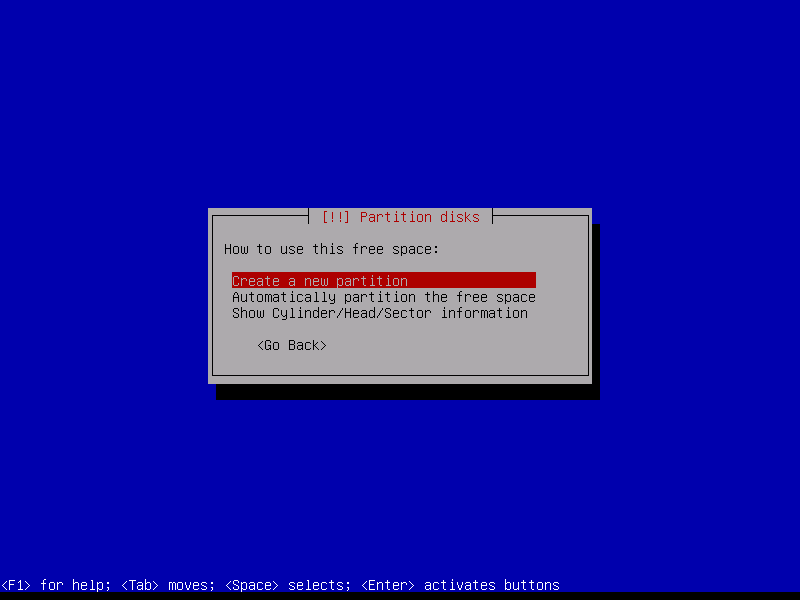
\includegraphics[width=0.85\textwidth]{screenshots/15_ubuntu_install.png}
\end{center}
\end{nofloat}

\pagebreak
Die Größenangabe kann hier ohne Änderungen übernommen werden.

\begin{nofloat}{figure}
\begin{center}
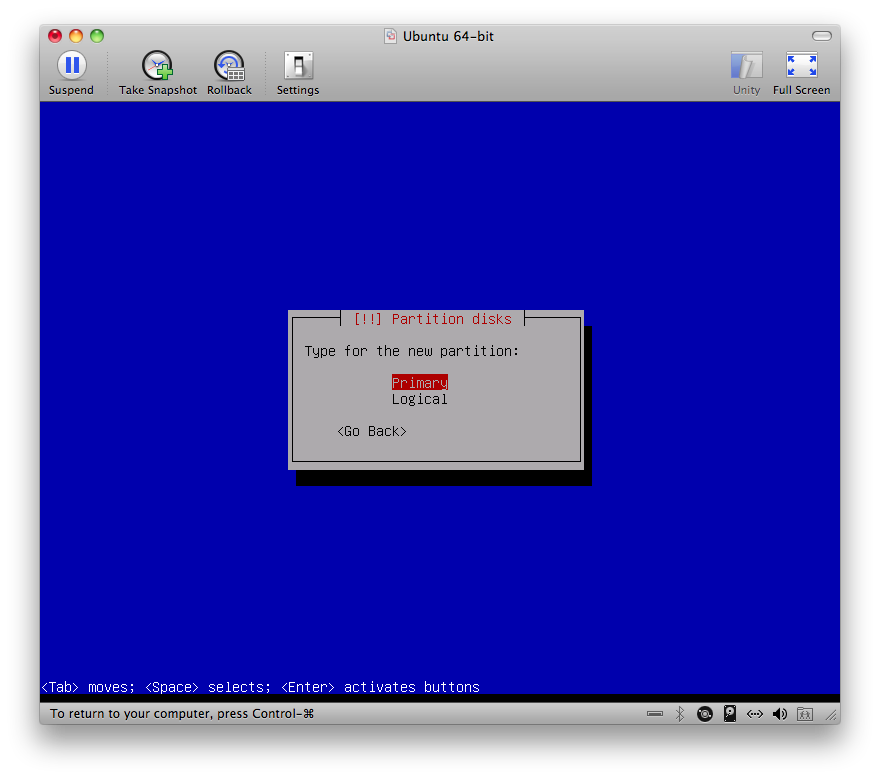
\includegraphics[width=0.85\textwidth]{screenshots/16_ubuntu_install.png}
\end{center}
\end{nofloat}

Wählen Sie hier wieder \textbf{Primär}.

\begin{nofloat}{figure}
\begin{center}
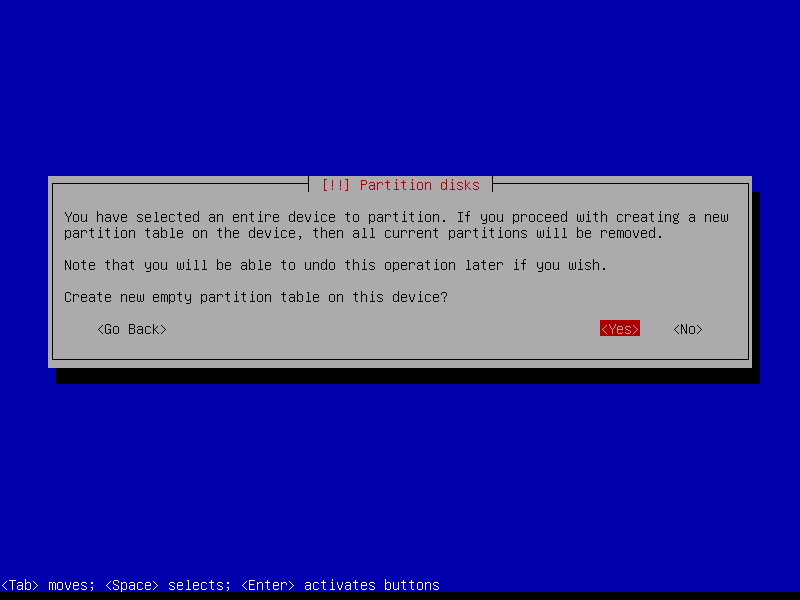
\includegraphics[width=0.85\textwidth]{screenshots/13_ubuntu_install.png}
\end{center}
\end{nofloat}

\pagebreak
Unter /textbf{Benutzen als:} wählen Sie nun \textbf{Auslagerungsspeicher (Swap)}.

\begin{nofloat}{figure}
\begin{center}
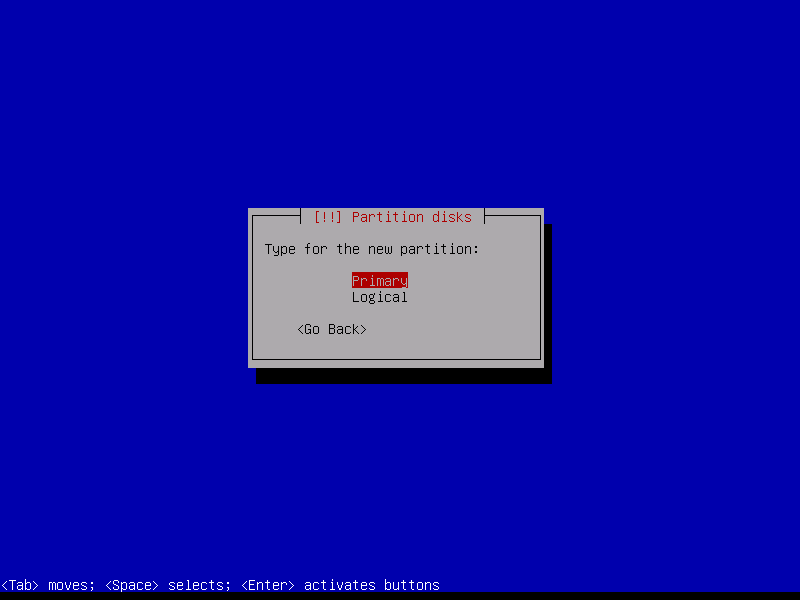
\includegraphics[width=0.85\textwidth]{screenshots/17_ubuntu_install.png}
\end{center}
\end{nofloat}

Hier wieder \textbf{Anlegen der Partition beenden} wählen.

\begin{nofloat}{figure}
\begin{center}
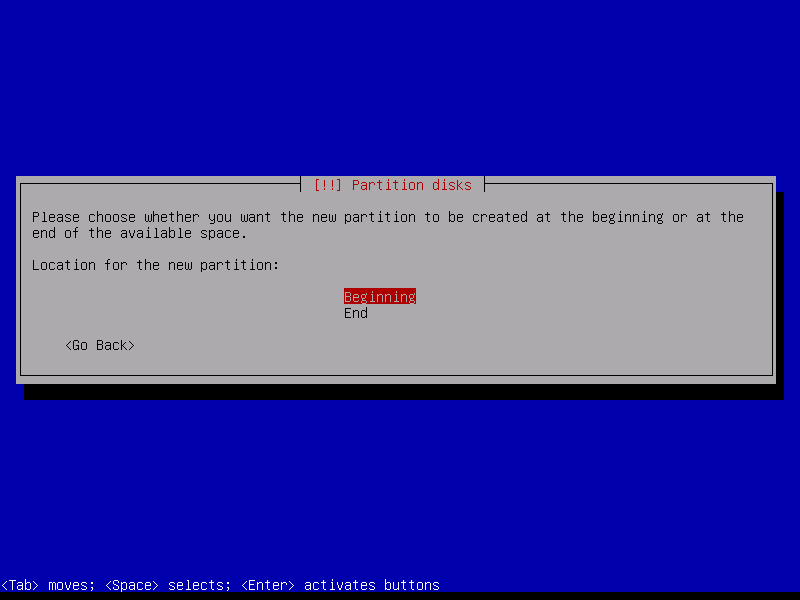
\includegraphics[width=0.85\textwidth]{screenshots/18_ubuntu_install.png}
\end{center}
\end{nofloat}

\pagebreak
Jetzt \textbf{Partitionierung beenden und Änderungen übernehmen} wählen.

\begin{nofloat}{figure}
\begin{center}
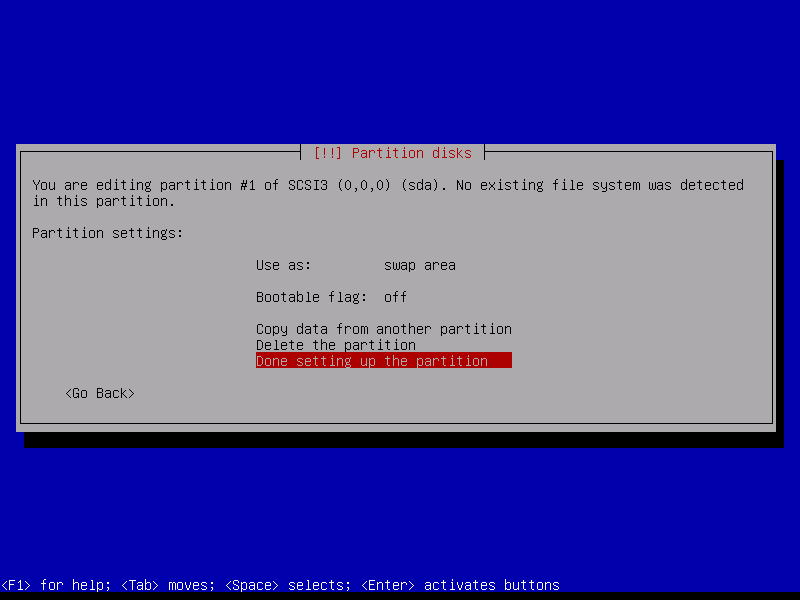
\includegraphics[width=0.85\textwidth]{screenshots/19_ubuntu_install.png}
\end{center}
\end{nofloat}

Hier \textbf{Ja} wählen.

\begin{nofloat}{figure}
\begin{center}
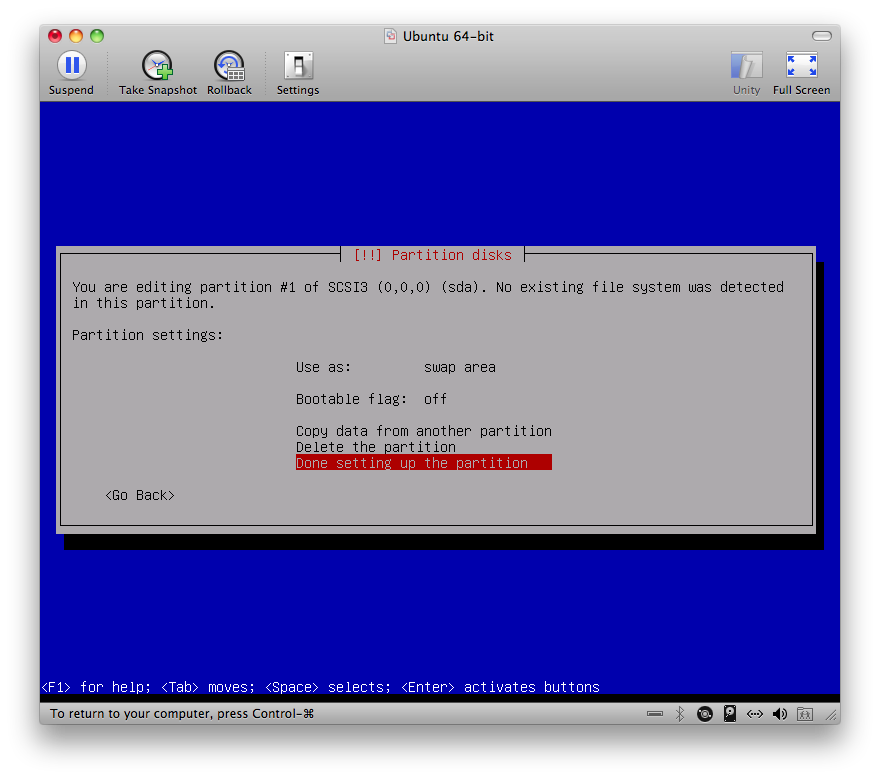
\includegraphics[width=0.85\textwidth]{screenshots/20_ubuntu_install.png}
\end{center}
\end{nofloat}

\pagebreak
Jetzt kann ein Benutzer angelegt werden. Für \textbf{srv1} wählen wir den Namen \textbf{admin1}.

\begin{nofloat}{figure}
\begin{center}
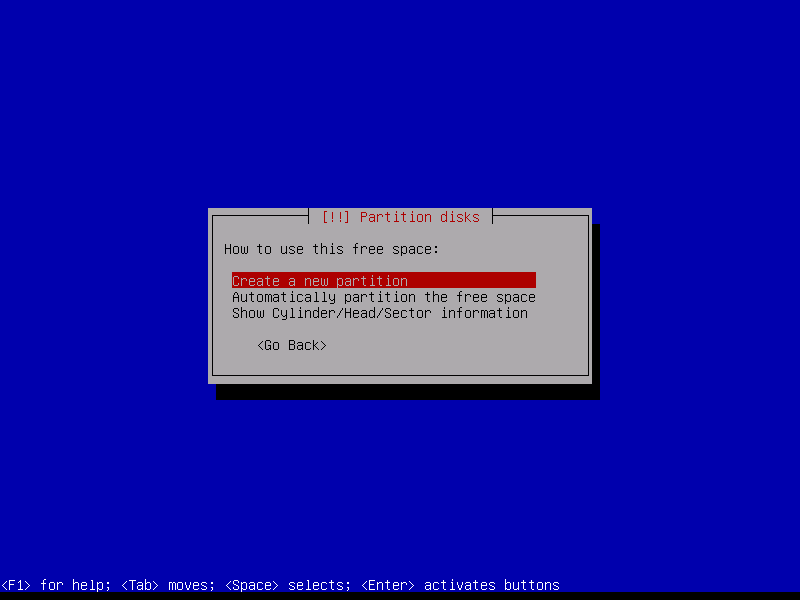
\includegraphics[width=0.85\textwidth]{screenshots/21_ubuntu_install.png}
\end{center}
\end{nofloat}

Der Benutzername soll auch \textbf{admin1} lauten.

\begin{nofloat}{figure}
\begin{center}
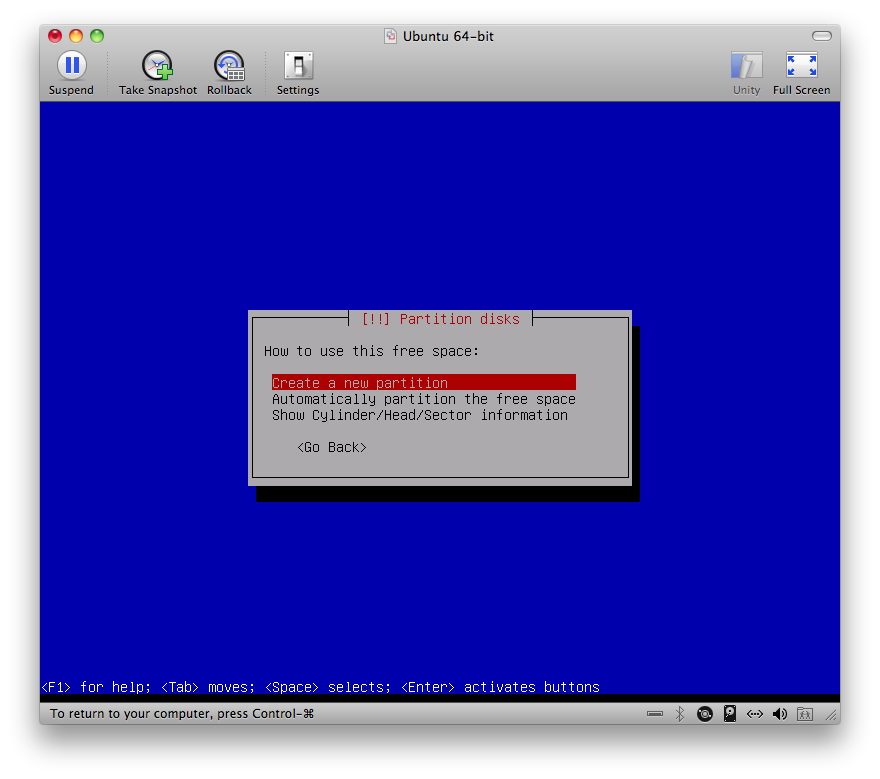
\includegraphics[width=0.85\textwidth]{screenshots/22_ubuntu_install.png}
\end{center}
\end{nofloat}

\pagebreak
Als Passwort vergeben wir hier \textbf{password1}.

\begin{nofloat}{figure}
\begin{center}
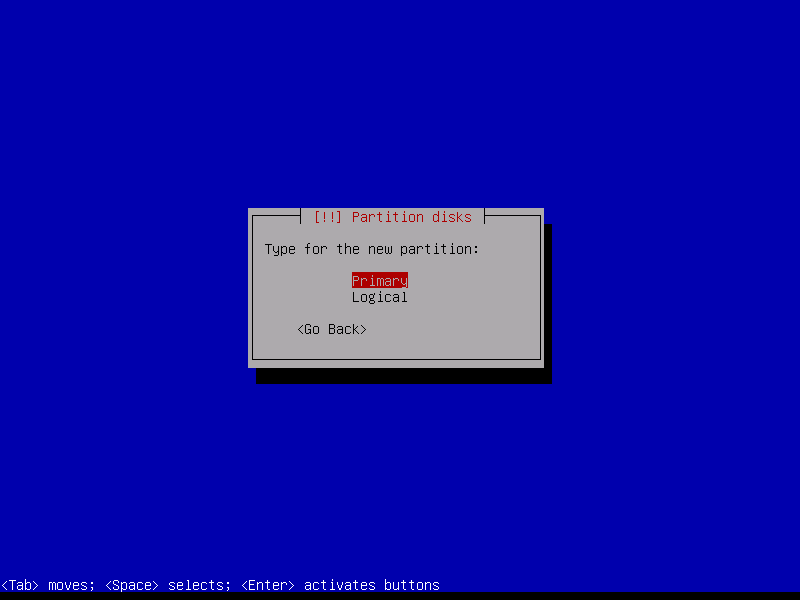
\includegraphics[width=0.85\textwidth]{screenshots/23_ubuntu_install.png}
\end{center}
\end{nofloat}

Die Verschlüsselung aktivieren wir nicht.

\begin{nofloat}{figure}
\begin{center}
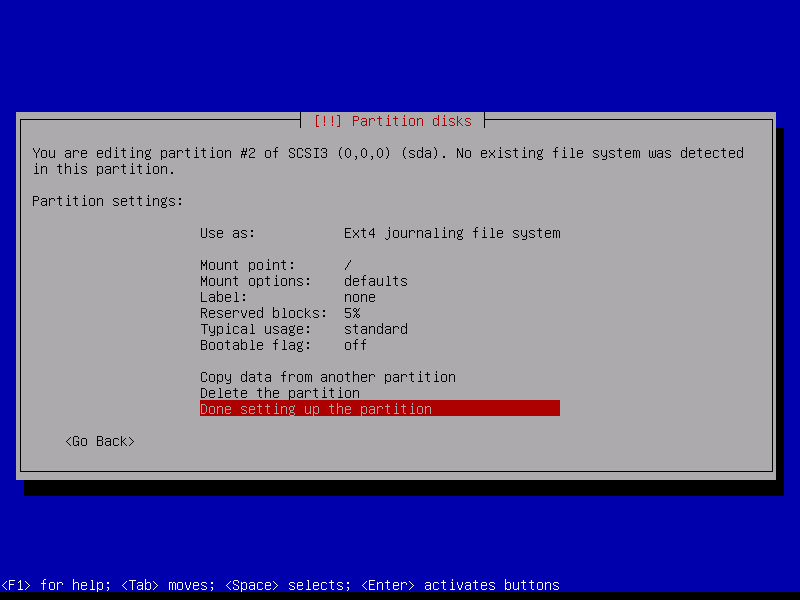
\includegraphics[width=0.85\textwidth]{screenshots/24_ubuntu_install.png}
\end{center}
\end{nofloat}

\pagebreak
Wir benötigen keinen HTTP-Proxy - daher einfach das Feld leer lassen
und mit der Eingabe-Taste bestätigen.

\begin{nofloat}{figure}
\begin{center}
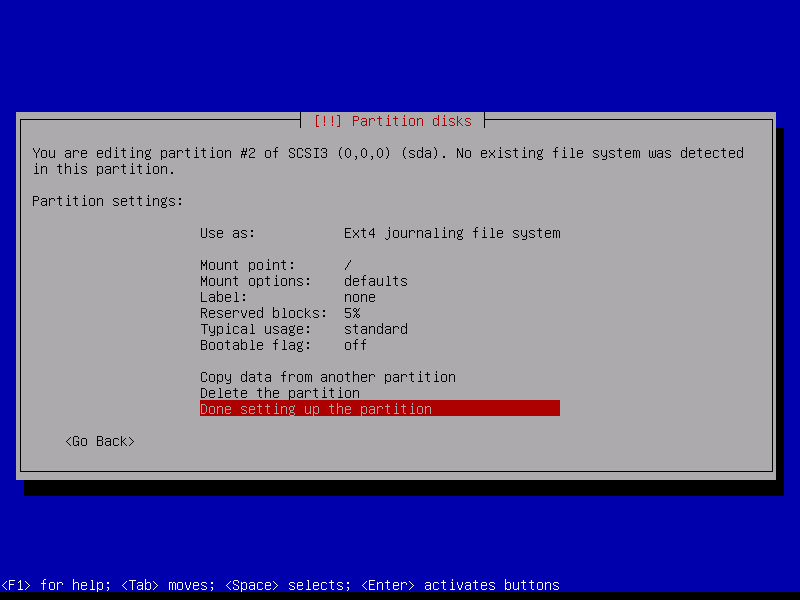
\includegraphics[width=0.85\textwidth]{screenshots/25_ubuntu_install.png}
\end{center}
\end{nofloat}

Wählen Sie hier \textbf{Keine automatischen Aktualisierungen}.

\begin{nofloat}{figure}
\begin{center}
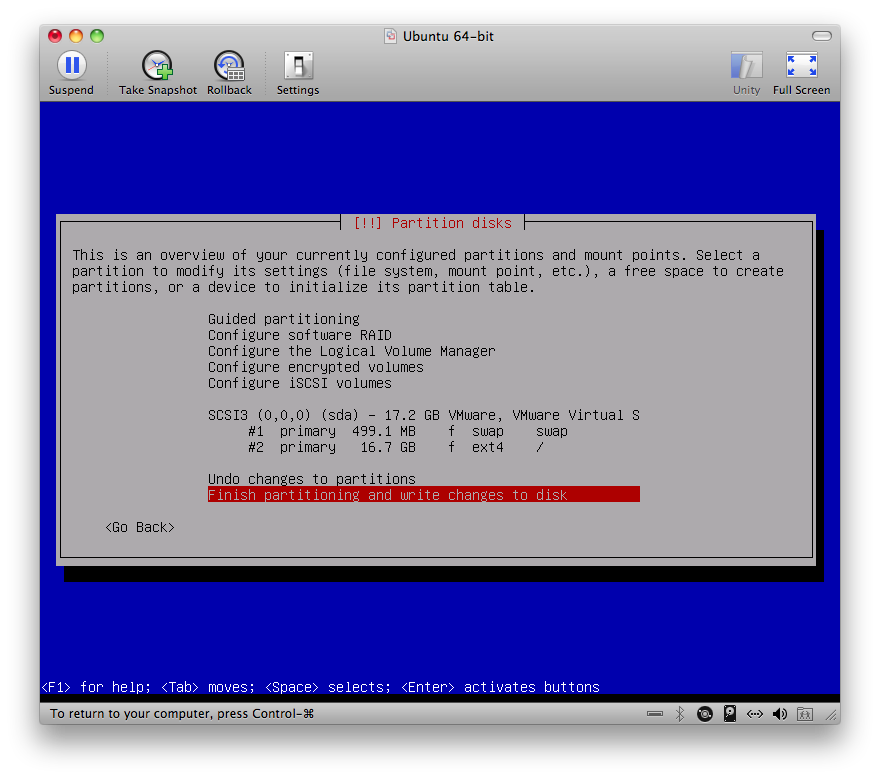
\includegraphics[width=0.85\textwidth]{screenshots/26_ubuntu_install.png}
\end{center}
\end{nofloat}

\pagebreak
Bei der zu installierenden Software wählen wir nur \textbf{OpenSSH server}.

\begin{nofloat}{figure}
\begin{center}
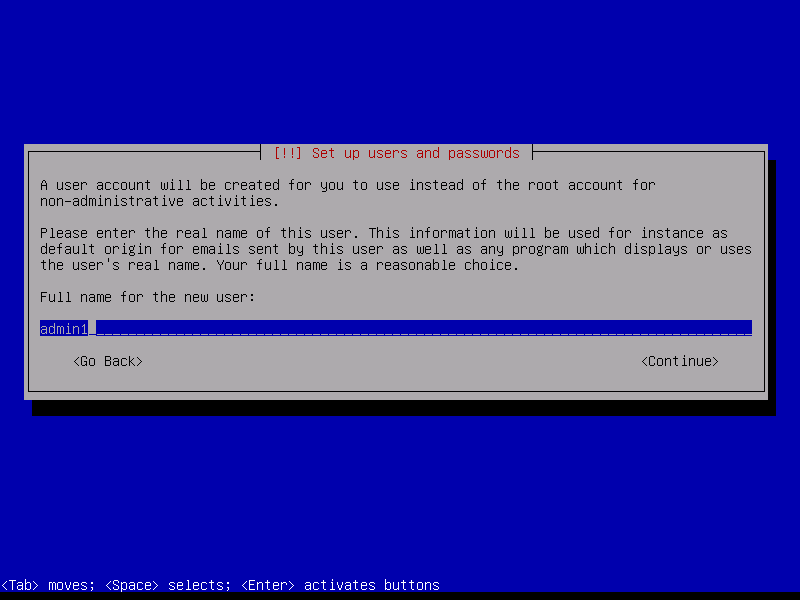
\includegraphics[width=0.85\textwidth]{screenshots/27_ubuntu_install.png}
\end{center}
\end{nofloat}

Nach der eigentlichen Installation wird nun der Bootloader installiert. Wählen Sie hier \textbf{Ja}.

\begin{nofloat}{figure}
\begin{center}
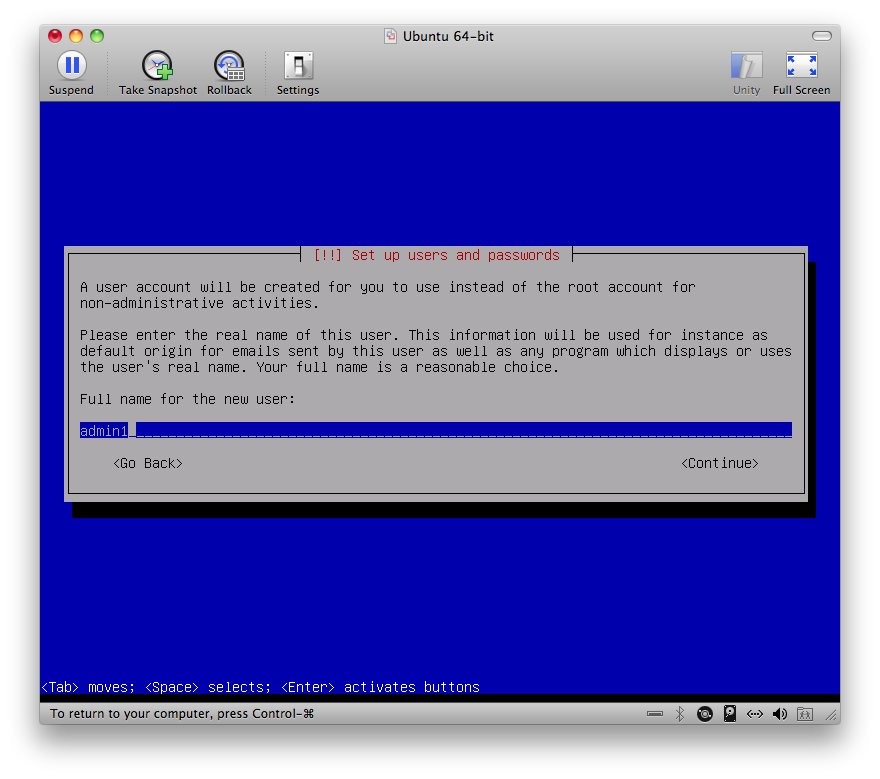
\includegraphics[width=0.85\textwidth]{screenshots/28_ubuntu_install.png}
\end{center}
\end{nofloat}

\pagebreak
Die Installation ist abgeschlossen. Hier einfach \textbf{Weiter} wählen. Die virtuelle Maschine startet nun neu und
bootet das neu installierte System.

\begin{nofloat}{figure}
\begin{center}
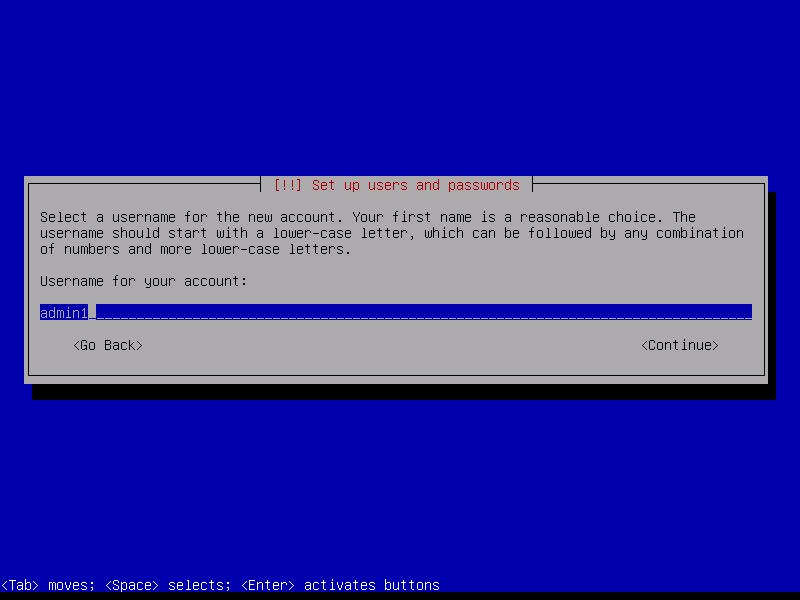
\includegraphics[width=0.85\textwidth]{screenshots/29_ubuntu_install.png}
\end{center}
\end{nofloat}

Verfahren Sie analog für den Server \textbf{srv2}.

\section{bind9, apache2 und postfix}

\subsection{Grundkonfiguration}

Im folgenden wird zunächst die Grundkonfiguration der Maschinen durchgeführt. Exemplarisch wird hier die Konfiguration für den Arbeitsplatz TK02 verwendet. Die für Sie
und Ihren Arbeitsplatz richtigen Werte entnehmen Sie bitte dem Anhang.

\subsubsection{Einrichtung IP-Adressen}

Melden Sie sich bei der Maschine \textbf{srv1} mit dem Benutzername \textbf{admin1} und dem Passwort \textbf{password1} an. Danach 
setzen Sie die korrekte IP-Adresse der virtuellen Maschine mit einem Texteditor Ihrer Wahl in der Datei \\
\textbf{/etc/network/interfaces}. Die Konfiguration für Ihre Arbeitsplatzrechner entnehmen Sie der entsprechenden Tabelle im Anhang. Hier wird exemplarisch die Konfiguration
von TK02 verwendet.

\begin{lstlisting}
admin1@srv1$ sudo vi /etc/network/interfaces
\end{lstlisting}
Eventuell werden Sie erneut zur Eingabe des Passwortes aufgefordert. Die Datei sollte danach folgenden Inhalt haben:


\begin{lstlisting}
# This file describes the network interfaces available on your system
# and how to activate them. For more information, see interfaces(5).

# The loopback network interface
auto lo
iface lo inet loopback

# The primary network interface
auto eth0
iface eth0 inet static
  address 10.174.26.202
  netmask 255.255.255.0
  gateway 10.174.26.254
  network 10.174.26.0
  broadcast 10.174.26.255
\end{lstlisting}

Jetzt sollte noch die Konfiguration der Namensauflösung in der Datei \\ \textbf{/etc/resolv.conf} angepasst werden. 
\begin{lstlisting}
admin1@srv1$ sudo vi /etc/resolv.conf
\end{lstlisting}

Diese Datei sollte danach folgenden Inhalt haben:
\begin{lstlisting}
nameserver 10.174.26.126
domain tknet02.informatik.hs-fulda.de
search tknet02.informatik.hs-fulda.de
\end{lstlisting}

\subsubsection{Update}
Jetzt sollte das System auf den neusten Stand gebracht werden. Geben Sie dazu folgende Befehle ein und bestätigen eventuell auftretende Rückfragen:
\begin{lstlisting}
admin1@srv1$ sudo apt-get update
admin1@srv1$ sudo apt-get upgrade
\end{lstlisting}
Starten Sie dann das System neu:
\begin{lstlisting}
admin1@srv1$ sudo init 6
\end{lstlisting}